% !TEX root = ../main.tex
\chapter{Визначення структури та оптимальних настройок регуляторів методом <<прямого>> синтезу}\label{ch:direct}
Розглядається об'єкт з передаточною функцією $W_{O_1}(s) = \frac{k e^{-\tau s}}{T_1 s + 1}$.
При перехідному режимі є бажаним аперіодичний перехідний процес в контурі цифрового керування,
тобто при подачі на задаюче діяння регулятора одиничного ступінчатого збурення
замкнений контур має вести себе як неперервна модель першого порядку з запізненням:
\begin{gather}
    W_{\text{з}}(s) = \frac{y(s)}{G(s)} = \frac{\lambda e^{-\tau s}}{s + \lambda}
\end{gather}

% да не хочу я это писать...

% З методичних рекомендацій маємо наступний вираз для ДПФ регулятора:
% \begin{gather}\label{reg_w01}
%     W_p(z) = \frac{
%         \left(1 - e^{-\lambda T_0}\right)
%         \left(1 - e^{-T_0 / T_1} z^{-1}\right)
%     }{
%         k
%         \left(1 - e^{-\lambda T_0} z^{-1} - \left(1 - e^{-\lambda T_0} z^{-d-1}\right) \right)
%         \left(C_1 + C_2 z^{-1}\right)
%     }
% \end{gather}
% де $a = 1 - \frac{\tau - d T_0}{T_0}$, $C_1 = 1 - e^{\frac{a T_0}{T_1}}$,
% $C_2 = e^{\frac{a T_0}{T_1}} - e^{\frac{T_0}{T_1}}$.


% Розглянемо характеристичне рівняння передаточної функції \eqref{reg_w01}:
% \begin{gather*}
%     \left(1 - e^{-\lambda T_0} z^{-1} - \left(1 - e^{-\lambda T_0} z^{-d-1}\right) \right)
%         \left(C_1 + C_2 z^{-1}\right) = 0
% \end{gather*}
% Якщо один з полюсів цього рівняння буде знаходитися в околі $z=-1$, то при аперіодичному перехідному процесі
% вихідної координати в замкненому контурі у керуючому діянні будуть коливальні процеси зі згасаючою амплітудою, які
% не є бажаними для виконавчого механізму. 
Згідно з методичними рекомендаціями, оптимальні параметри ПІ-регулятора з ДПФ 
$K_p \left(
    1 + \frac{T_0}{T_I \left(1 - z^{-1}\right)}
\right)$
визначаються за формулами
\begin{gather}\label{K_p_opt__direct}
    K_{p_{\text{опт}}} = \frac{
        1 - e^{-\lambda T_0}
    }{
        k \left(e^{T_0 / T_1} - 1\right) \left(1 + d \left(1 - e^{-\lambda T_0}\right)\right)
    } \\ \label{T_I_opt__direct}
    T_{I_{\text{опт}}} = \frac{T_0}{e^{T_0 / T_1} - 1}
\end{gather}
де $d$ -- ціла частина від ділення часу запізнення $\tau$ на період квантування
$T_0$, який беремо на основі умови забезпечення необхідної точності керування.
Візьмемо $T_0 = 0.1127$. Тоді $d = 124$, $T_{I_{\text{опт}}} = 34.9437$, а для різних варіантів $\lambda$ отримаємо такі значення $K_{p_{\text{опт}}}$:
\begin{center}
    \begin{tabular}{|c|c|}
        \hline
        $\lambda$ & $K_{p_{\text{опт}}}$ \\
        \hline
        $\frac{1}{T_1} \approx 0.0286$      & $0.0765$ \\
        \hline
        $\frac{1}{1.5T_1} \approx 0.0190$   & $0.0564$ \\
        \hline
        $\frac{1}{2T_1} \approx 0.0143$     & $0.0446$ \\
        \hline
        $\frac{1}{3T_1} \approx 0.0095$     & $0.0315$ \\
        \hline
    \end{tabular}
\end{center}
Для цифрового моделювання перехідних процесів в замкненому контурі цифрового керування зауважимо, що
можна записати рівняння
\begin{gather*}
    y(z) = W_p(z) W_{\text{п}}(z) \left(G(z) - y(z)\right) \Rightarrow
    y(z) = \frac{W_p(z) W_{\text{п}}(z)}{1 + W_p(z) W_{\text{п}}(z)} G(z) = W_{\text{з}}(z) G(z)
\end{gather*}
де $y(z)$, $G(z)$ -- $z$-перетворення від керованої координати і задаючого діяння відповідно, а 
передаточну функцію $W_{\text{з}}(z)$ було обчислено в \eqref{W_3_for_direct}.
Можна записати рекурентне рівняння, за яким буде відбуватися моделювання:
\begin{gather}
    \mbox{\small $y_n = \left(1 + e^{-T_0/T_1}\right) y_{n-1} - e^{-T_0/T_1} y_{n-2} - $} \nonumber \\
    \mbox{\small $-
    \frac{k K_{p_{\text{опт}}}}{T_I} \left(
        \left(C_1 T_{I_{\text{опт}}} + C_1 T_0\right) y_{n-d-1} + 
        \left(-C_1 T_{I_{\text{опт}}} + C_2 T_{I_{\text{опт}}} + C_2 T_0\right) y_{n-d-2} -
        C_2 T_{I_{\text{опт}}} y_{n-d-3}
    \right) +$} \nonumber \\
    \mbox{\small $+ \frac{k K_{p_{\text{опт}}}}{T_I} \left(
        \left(C_1 T_{I_{\text{опт}}} + C_1 T_0\right) g_{n-d-1} + 
        \left(-C_1 T_{I_{\text{опт}}} + C_2 T_{I_{\text{опт}}} + C_2 T_0\right) g_{n-d-2} -
        C_2 T_{I_{\text{опт}}} g_{n-d-3}
    \right)$}
\end{gather}
де $a = 1 - \frac{\tau - d T_0}{T_0}$, $C_1 = 1 - e^{-\frac{a T_0}{T_1}}$,
$C_2 = e^{-\frac{a T_0}{T_1}} - e^{-\frac{T_0}{T_1}}$, початкові умови для $y$ нульові,
а $g_n = 1$.
Отже, маємо наступні перехідні процеси для різних значень $\lambda$:
\begin{center}
    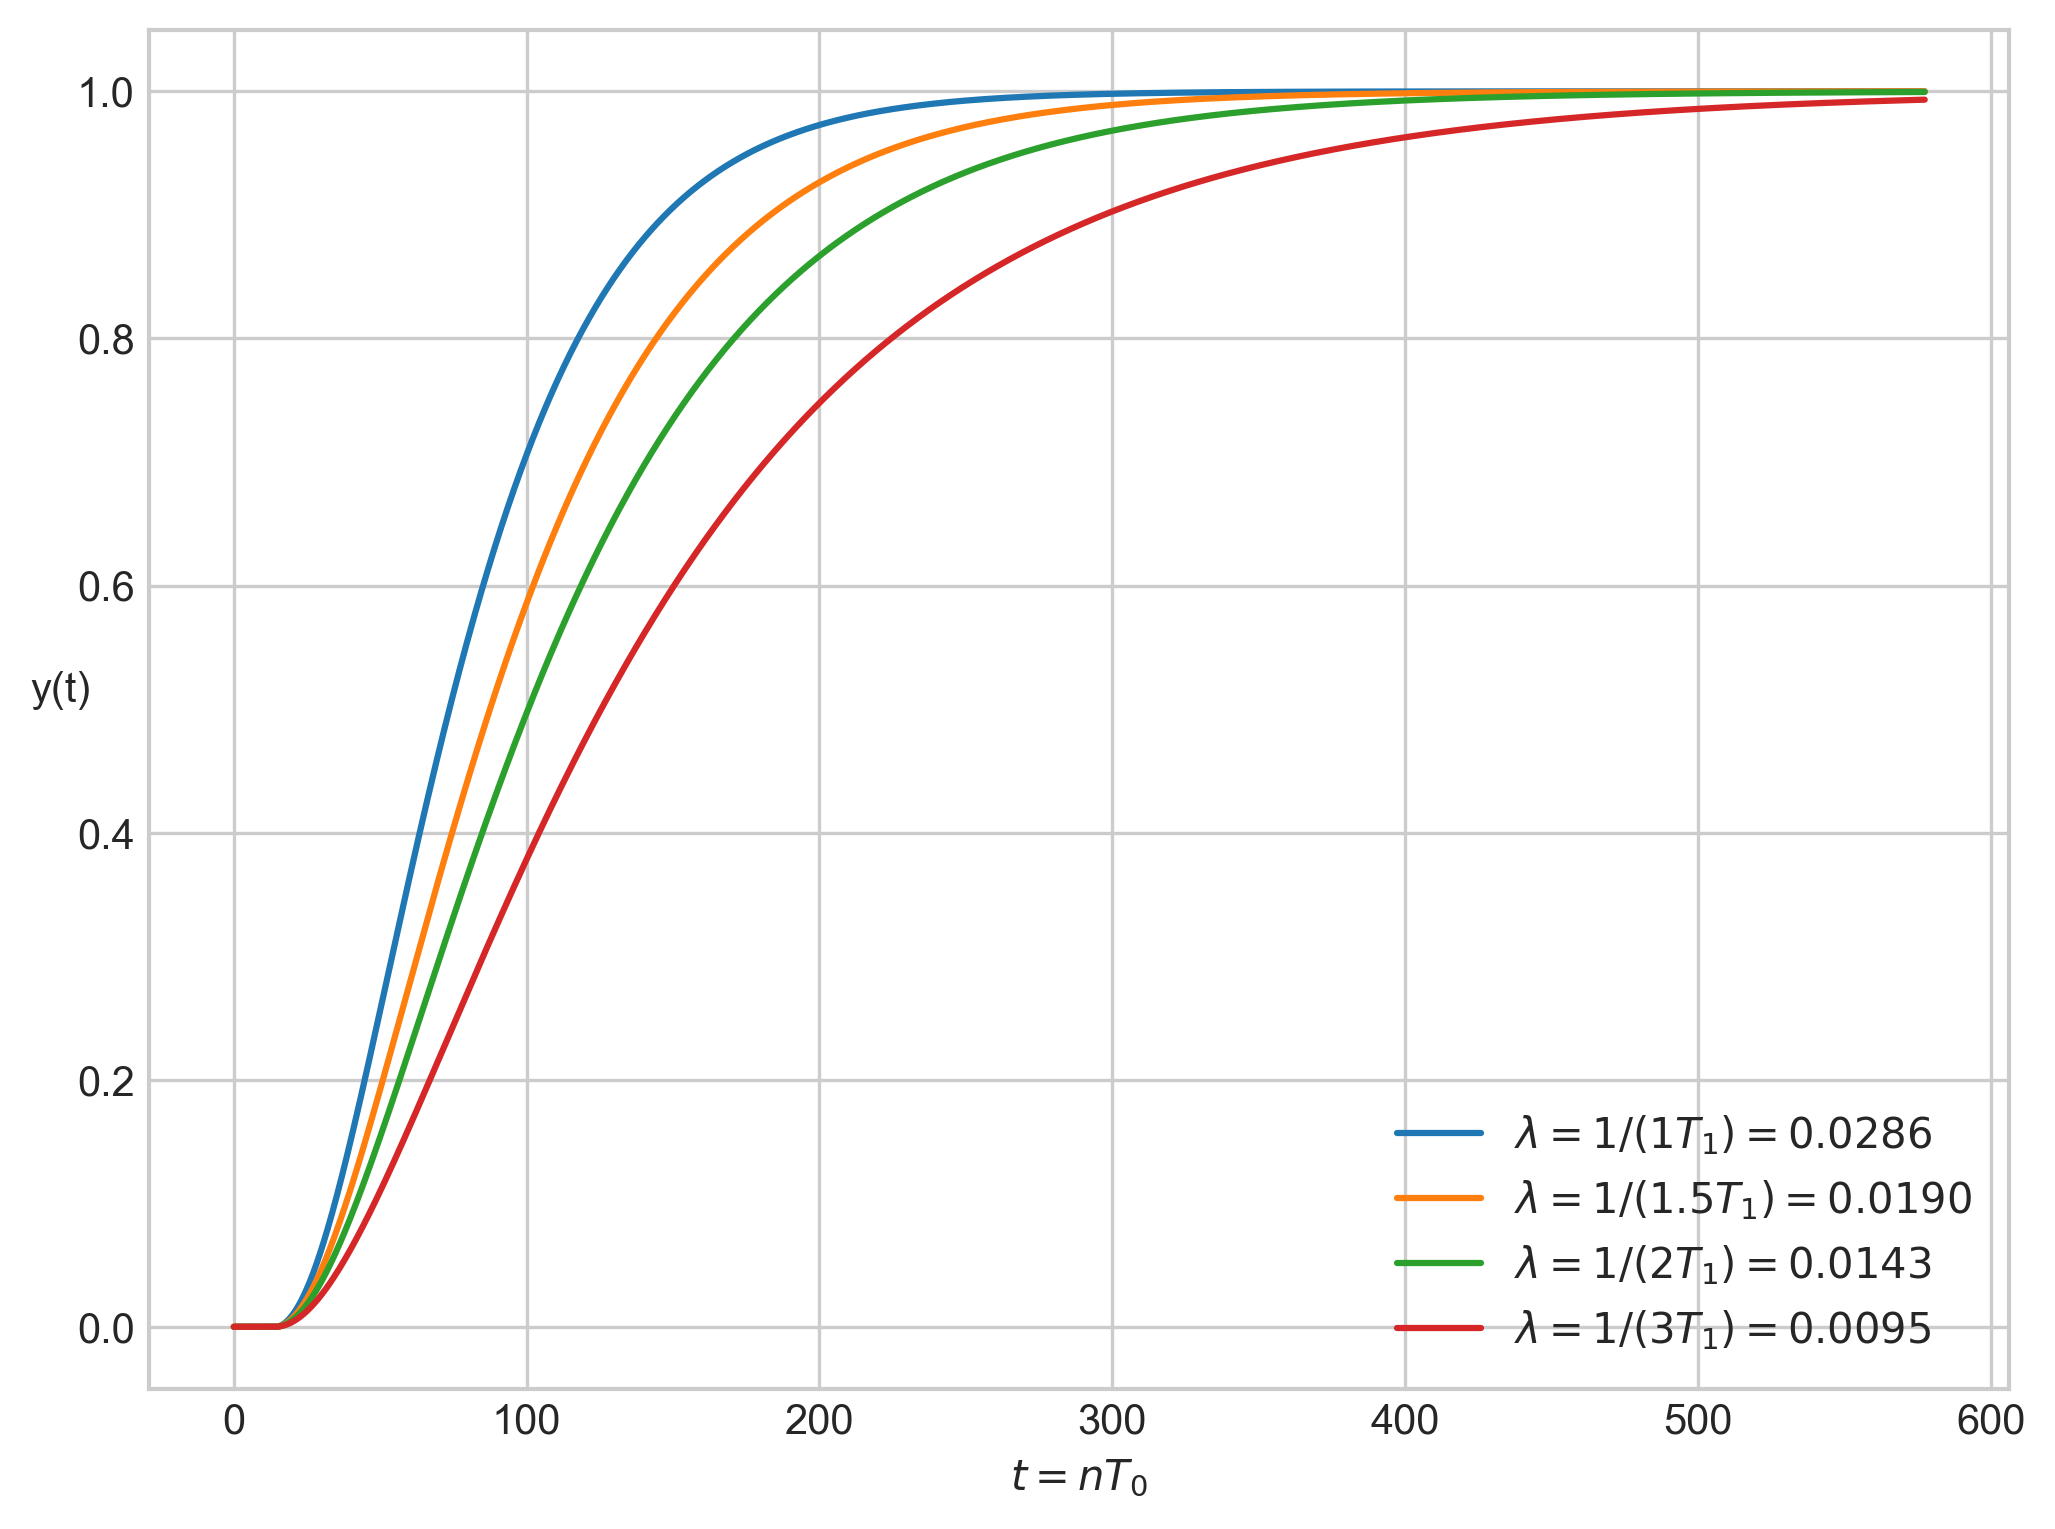
\includegraphics{pics/transient_process_task_4.png}
\end{center}
Видно, що процес зміни вихідної координати дійсно має бажаний аперіодичний характер.

На основі формул \eqref{K_p_opt__direct} та \eqref{T_I_opt__direct} можна визначити
оптимальні настройки для неперервного регулятора, взявши границі при $T_0 \to 0$. Отримаємо
$K_p^H = \frac{\lambda T_1}{k \left(1 + \lambda \tau\right)}$, $T_I^H = T_1$.